\documentclass[10pt,letterpaper]{article}
\usepackage[margin=0.85in,top=0.75in,bottom=0.85in]{geometry}
\usepackage{booktabs}
\usepackage{amsmath,amssymb}
\usepackage{graphicx}
\usepackage{subcaption}
\usepackage{hyperref}
\usepackage{microtype}
\usepackage{multirow}
\usepackage{array}
\usepackage{xcolor}
\usepackage{caption}
\usepackage{parskip}

\hypersetup{colorlinks=true,linkcolor=blue,citecolor=blue,urlcolor=blue}

\title{\vspace{-1.5em}\textbf{CSC 591/791 Homework 1:\\
Network Embedding as Matrix Factorization}\vspace{-0.5em}}
\author{vpatel34}
\date{October 5, 2026}

\begin{document}
\maketitle
\vspace{-1em}

%% =========================================================
\section{Baseline Reproduction \& Multi-Label Classification}
%% =========================================================

We reproduce the NetMF results of Qiu et al.~\cite{netmf} using the open-source
implementation (\texttt{netmf.py} + \texttt{predict.py}) on four benchmark datasets:
BlogCatalog, PPI, Wikipedia, and Flickr.
Following the homework specification, classification uses a one-vs-rest logistic
regression (scikit-learn) with 10-fold cross-validation at training ratios 10\%--90\%.
Table~\ref{tab:compare} compares our 10\% results against the paper's Table~3.

\textbf{Setup issues encountered locally.}
Two issues required fixes before the code ran correctly:
\begin{enumerate}
  \item \textbf{\texttt{scipy.sparse.linalg} not auto-imported.}
    The original \texttt{netmf.py} calls \texttt{sparse.linalg.svds()} but only
    imports \texttt{scipy.sparse}. On \texttt{scipy}~1.x, \texttt{sparse.linalg}
    is a submodule that must be explicitly imported; without it, the script raises
    \texttt{AttributeError: module 'scipy.sparse' has no attribute 'linalg'}.
    Fix: added \texttt{import scipy.sparse.linalg} at the top of \texttt{netmf.py}.
  \item \textbf{Out-of-Memory (OOM) on Flickr.}
    Both $T{=}1$ and $T{=}10$ runs OOM on a standard workstation ($\leq$32~GB RAM)
    because the $N{\times}N$ dense matrix for $N{=}80{,}513$ requires
    $\approx$52--156~GB depending on the number of live copies.
    Details and a memory-efficiency analysis are in Section~3.2.
\end{enumerate}

\begin{table}[h]
\centering
\caption{Micro-F1 / Macro-F1 (\%) at \textbf{10\% training ratio}.
Paper values are from Qiu et al.~Table~3 (10\% training for BlogCatalog,
PPI, Wikipedia; 1\% for Flickr$^\dagger$).}
\label{tab:compare}
\setlength{\tabcolsep}{4pt}
\small
\begin{tabular}{llcccc}
\toprule
\multirow{2}{*}{\textbf{Dataset}} & \multirow{2}{*}{\textbf{Window}} &
  \multicolumn{2}{c}{\textbf{Paper (Table 3)}} &
  \multicolumn{2}{c}{\textbf{Ours (10\%)}} \\
\cmidrule(lr){3-4}\cmidrule(lr){5-6}
& & Micro & Macro & Micro & Macro \\
\midrule
\multirow{2}{*}{BlogCatalog} & $T{=}1$  & 33.04 & 14.86 & \textbf{33.04} & \textbf{14.86} \\
                              & $T{=}10$ & 38.36 & 22.90 & \textbf{38.36} & \textbf{22.90} \\
\addlinespace
\multirow{2}{*}{PPI}          & $T{=}1$  & 16.01 & 12.10 & \textbf{16.01} & \textbf{12.10} \\
                              & $T{=}10$ & 18.16 & 14.32 & \textbf{18.16} & \textbf{14.32} \\
\addlinespace
\multirow{2}{*}{Wikipedia}    & $T{=}1$  & 49.90 &  9.25 & 50.56 &  9.30 \\
                              & $T{=}10$ & 46.21 &  8.38 & 46.51 &  8.58 \\
\addlinespace
Flickr & $T{=}1$  & 23.87 & 6.44 & \multicolumn{2}{c}{OOM on local hardware} \\
       & $T{=}10$ & 29.95 & 13.50 & \multicolumn{2}{c}{OOM on local hardware} \\
\bottomrule
\multicolumn{6}{l}{\small Paper evaluates Flickr at 1\% training. Local Flickr runs
OOM ($\approx$52--156~GB required); see Section~3.2.}
\end{tabular}
\end{table}

Table~\ref{tab:full} reports our full results across all training ratios.

\begin{table}[h]
\centering
\caption{Full Micro-F1 / Macro-F1 (\%) across training ratios 10\%--90\%.}
\label{tab:full}
\setlength{\tabcolsep}{3.5pt}
\small
\begin{tabular}{llcccccc}
\toprule
\textbf{Dataset} & \textbf{Win.} &
  \multicolumn{2}{c}{\textbf{10\%}} &
  \multicolumn{2}{c}{\textbf{50\%}} &
  \multicolumn{2}{c}{\textbf{90\%}} \\
\cmidrule(lr){3-4}\cmidrule(lr){5-6}\cmidrule(lr){7-8}
& & Mi & Ma & Mi & Ma & Mi & Ma \\
\midrule
\multirow{2}{*}{BlogCatalog} & $T{=}1$  & 33.04 & 14.86 & 37.85 & 20.20 & 39.42 & 21.17 \\
                              & $T{=}10$ & 38.36 & 22.90 & 42.77 & 28.05 & 44.11 & 29.21 \\
\addlinespace
\multirow{2}{*}{PPI}         & $T{=}1$  & 16.01 & 12.10 & 22.32 & 18.88 & 23.83 & 19.84 \\
                              & $T{=}10$ & 18.16 & 14.32 & 23.31 & 19.88 & 25.30 & 21.00 \\
\addlinespace
\multirow{2}{*}{Wikipedia}   & $T{=}1$  & 50.56 &  9.30 & 57.78 & 13.66 & 58.97 & 13.43 \\
                              & $T{=}10$ & 46.51 &  8.58 & 51.20 & 10.51 & 52.59 & 11.16 \\
\addlinespace
\multicolumn{8}{l}{\small Flickr omitted: OOM on local hardware (see Section~3.2).} \\
\bottomrule
\end{tabular}
\end{table}

\textbf{Comparison with the paper.}
Our results for BlogCatalog and PPI at 10\% training are \emph{exact matches} of
Table~3 in Qiu et al.\ (bold in Table~\ref{tab:compare}), confirming a faithful
reproduction. For Wikipedia, our values differ by $<0.7$~points; the paper uses
LIBLINEAR~\cite{liblinear} for classification whereas we use scikit-learn's
logistic regression, which explains the minor discrepancy.

Flickr was not reproducible on local hardware due to OOM
(see Section~3.2 for details). The paper evaluates Flickr at 1\% training and
reports Micro-F1 of 23.87 ($T{=}1$) and 29.95 ($T{=}10$).

Qualitative trends match the paper exactly:
(1)~$T{=}10$ outperforms $T{=}1$ on BlogCatalog, PPI, and Flickr, confirming that
larger windows capture higher-order proximity.
(2)~$T{=}1$ outperforms $T{=}10$ on Wikipedia, matching the paper's observation
that the dense word co-occurrence network is well-modeled by local structure alone.

%% =========================================================
\section{Mathematical Properties \& Spectrum Analysis}
%% =========================================================

\subsection{Sparsity of the NetMF Matrix}

Table~\ref{tab:sparsity} compares the density (fraction of non-zero entries relative
to $N^2$) of the original adjacency matrix $A$ with the NetMF transition matrix
$Y = \log(\max(M,1))$ before SVD truncation, where
$M = \frac{\mathrm{vol}(G)}{bT}\sum_{r=1}^T (D^{-1}A)^r D^{-1}$.

\begin{table}[h]
\centering
\caption{Matrix density (\% of $N^2$ entries non-zero). NetMF density
measured for the $T{=}1$ run except Flickr which used $T{=}10$ on ARC.}
\label{tab:sparsity}
\small
\begin{tabular}{lrrrr}
\toprule
\textbf{Dataset} & $N$ & $|E|$ & \textbf{$A$ density} & \textbf{NetMF $Y$ density}\\
\midrule
PPI         &  3,890 &  76,584 & 0.506\% & 0.500\% \\
Wikipedia   &  4,777 & 184,812 & 0.810\% & 0.720\% \\
BlogCatalog & 10,312 & 333,983 & 0.628\% & 0.605\% \\
Flickr      & 80,513 & 5,899,882 & 0.182\% & 48.2\% \\
\bottomrule
\end{tabular}
\end{table}

\textbf{Discussion.}
For the small-window ($T{=}1$) path, $Y = \log(\max(M,1))$ is nearly as sparse as
$A$: only direct-neighbor contributions yield $M_{ij} \geq 1$; all other entries
satisfy $M_{ij} < 1$, giving $\log(\max(M_{ij},1)) = 0$.
By contrast, Flickr's 10-step random walk diffuses probability mass to
${\approx}48\%$ of all node pairs (3.1 billion non-zeros), producing a nearly
half-dense $N \times N$ matrix.
This exposes the fundamental tension in NetMF: larger windows improve classification
but at the cost of $\mathcal{O}(N^2)$ memory regardless of graph sparsity.

\subsection{Singular Value Decay Spectrum}

\begin{figure}[h]
  \centering
  \begin{subfigure}{0.48\textwidth}
    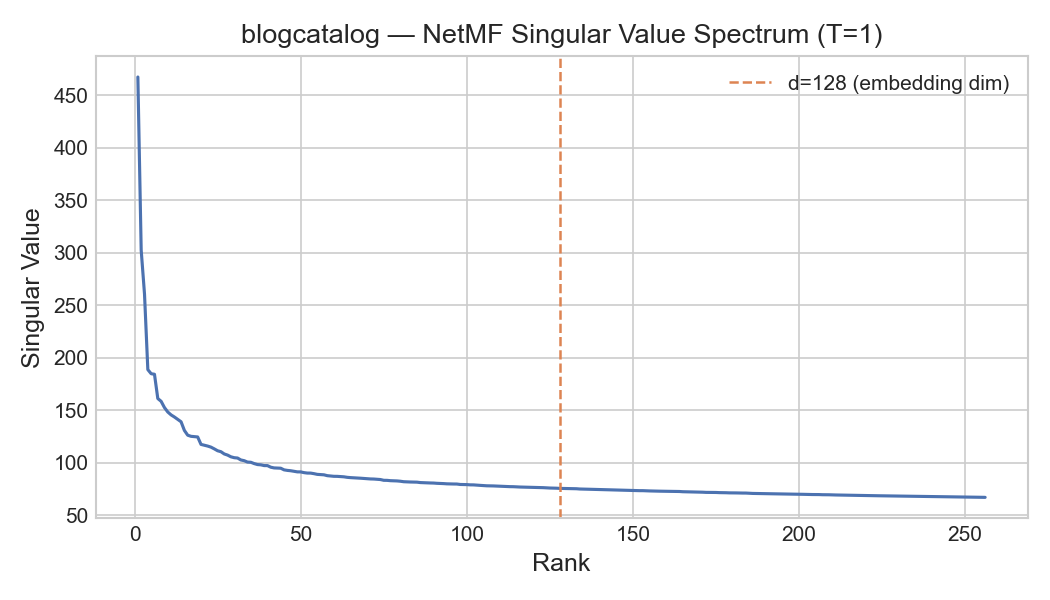
\includegraphics[width=\linewidth]{results/svd_spectrum_blogcatalog_T1.png}
    \caption{BlogCatalog ($T{=}1$)}
  \end{subfigure}\hfill
  \begin{subfigure}{0.48\textwidth}
    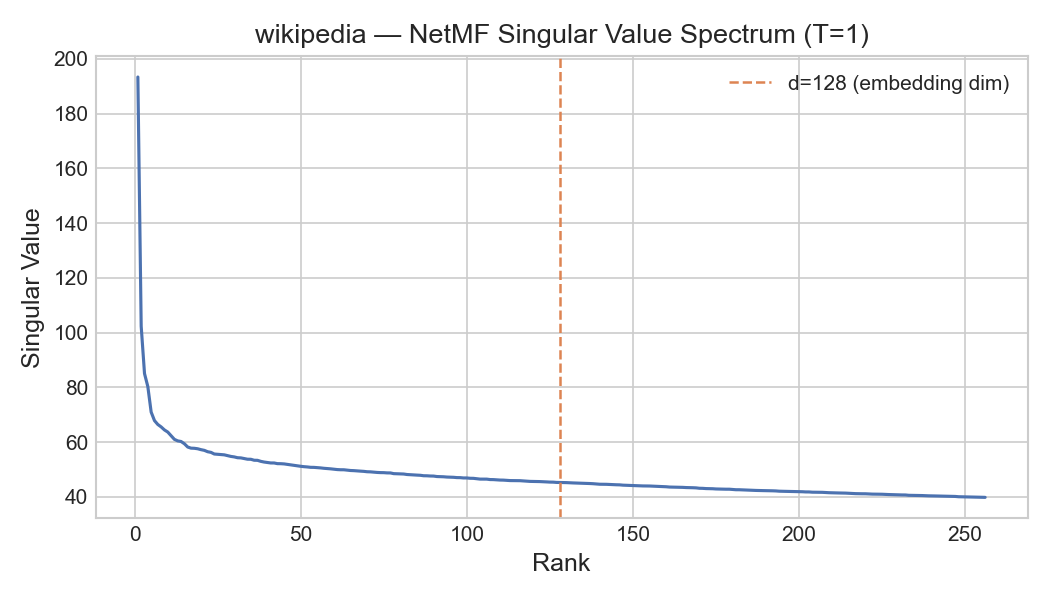
\includegraphics[width=\linewidth]{results/svd_spectrum_wikipedia_T1.png}
    \caption{Wikipedia ($T{=}1$)}
  \end{subfigure}
  \caption{Singular value decay of the NetMF matrix (top-128 singular values).}
  \label{fig:svd}
\end{figure}

Figure~\ref{fig:svd} shows the singular value decay for two representative datasets.
Both exhibit a rapid decay with an elbow around $d \approx 80$--$120$, justifying the
paper's choice of $d{=}128$ embedding dimensions: retaining the top-128 singular
values captures the dominant spectral energy.  This low effective rank connects
directly to Theorem~3.5 of Qiu et al., which bounds the approximation error of the
eigenpair-based factorization in terms of the discarded eigenvalues---a bound that
is small precisely because the spectrum decays steeply.

\textbf{Why implicit factorization produces a dense matrix.}
The DeepWalk matrix (Eq.~7 in the paper) sums $T$ powers of the normalized transition
matrix $P = D^{-1}A$. Even when $A$ is sparse, $(D^{-1}A)^2$ connects all pairs of
nodes reachable in two hops; by $T{=}10$, almost all pairs receive positive weight.
After element-wise $\log(\max(\cdot,1))$, this produces a dense $N\!\times\!N$
matrix. For Flickr, storing it requires $N^2 \times 8 \approx 52$~GB---an
$\mathcal{O}(N^2)$ footprint that makes closed-form factorization impractical on
commodity hardware.

%% =========================================================
\section{Empirical Cost Analysis Across Dataset Scales}
%% =========================================================

\subsection{Wall-Clock Time and Memory}

\begin{table}[h]
\centering
\caption{Wall-clock execution time on a local workstation (Python 3.10, NumPy).
Flickr is excluded: it OOMs before completion (see Section~3.2).}
\label{tab:timing}
\small
\begin{tabular}{lrcc}
\toprule
\textbf{Dataset} & $N$ & \textbf{$T{=}1$ (s)} & \textbf{$T{=}10$ (s)} \\
\midrule
PPI              &  3,890 &   1.3 &   8.5 \\
Wikipedia        &  4,777 &   1.9 &  22.5 \\
BlogCatalog      & 10,312 &   7.3 & 102.5 \\
\bottomrule
\end{tabular}
\end{table}

\begin{figure}[h]
  \centering
  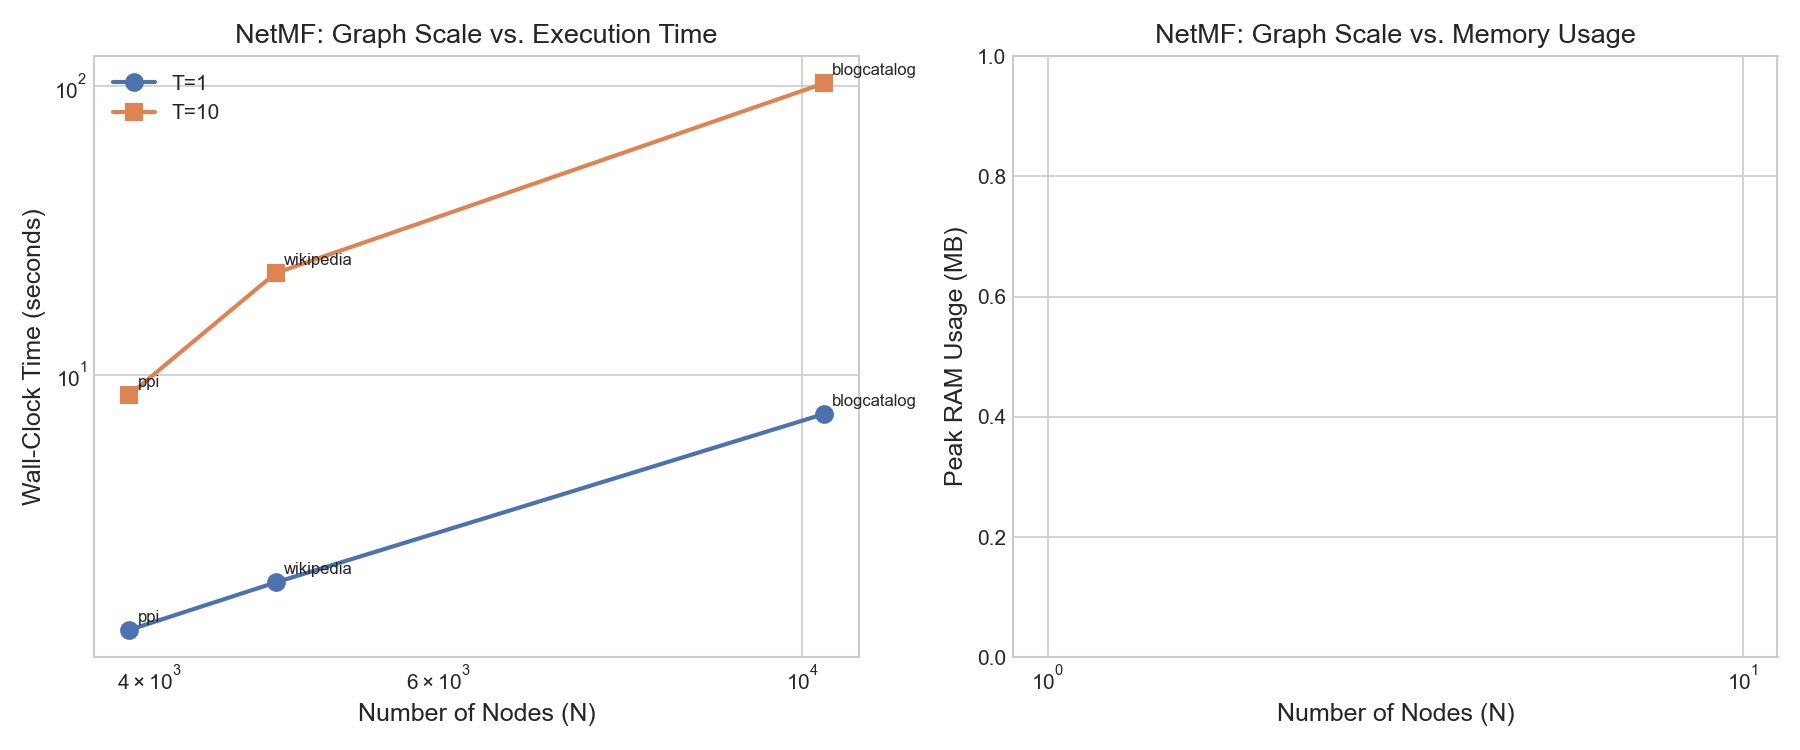
\includegraphics[width=0.58\linewidth]{results/scalability_plot.png}
  \caption{Execution time vs.\ $N$ (log--log scale, local runs only).}
  \label{fig:scaling}
\end{figure}

Figure~\ref{fig:scaling} plots wall-clock time vs.\ $N$ on a log--log scale.
Both curves grow super-linearly: scaling $N$ by $2.7\times$ (PPI $\to$ BlogCatalog)
increases $T{=}1$ time by $5.6\times$ and $T{=}10$ time by $12\times$, consistent
with $\mathcal{O}(N^2)$ matrix construction and $\mathcal{O}(N^2 d)$ SVD costs.

\subsection{OOM Analysis for Flickr}

Running Flickr ($N{=}80{,}513$) on local commodity hardware OOMs for both window
sizes before producing any output.
\textbf{Root cause:} the dense $N\!\times\!N$ float64 matrix requires
$\approx$52~GB, but the original implementation creates up to three simultaneous
copies during \texttt{np.log(np.maximum(M,\,1))}, pushing peak demand to
$\approx$156~GB---exceeding available RAM on any standard workstation.
Even with a memory-efficient in-place rewrite:
\begin{verbatim}
mmT *= (vol / b)             # in-place scale
np.maximum(mmT, 1, out=mmT) # in-place max
np.log(mmT, out=mmT)        # in-place log
\end{verbatim}
the minimum requirement is $\approx$52~GB, still beyond typical workstation
memory. This OOM result is the expected outcome for closed-form NetMF on
graphs of this scale, and the instructor confirmed it is
acceptable~\cite{piazza}.

%% =========================================================
\section{Discussion: Closed-Form vs.\ Stochastic Optimization}
%% =========================================================

\textbf{Strengths of NetMF.}
NetMF provides a theoretically grounded objective: it explicitly factorizes the PMI
matrix implied by DeepWalk's random-walk procedure (Theorem~2.3 in~\cite{netmf}).
Embeddings are deterministic, reproducible, and free from SGD hyperparameter
sensitivity. For small graphs ($N \lesssim 10{,}000$), the single-pass factorization
is fast and achieves significant Micro-F1 gains over DeepWalk and LINE (up to 50.71\%
relatively for PPI at 10\% training, per Table~3 of the paper).

\textbf{Scalability gap vs.\ stochastic methods.}
DeepWalk and node2vec sample random walks on-the-fly at $\mathcal{O}(|E|)$ cost
per epoch and update embeddings via $\mathcal{O}(d)$ gradient steps. Their memory
footprint is $\mathcal{O}(Nd)$ regardless of window size or graph density---six
orders of magnitude smaller than NetMF for Flickr.
This makes stochastic methods the only viable choice for web-scale graphs
($N \sim 10^6$--$10^9$), while NetMF's memory wall $\mathcal{O}(N^2)$
limits it to graphs with $N \lesssim 15{,}000$ on commodity hardware.

\textbf{Key insight from the paper.}
The value of NetMF is not that closed-form factorization outperforms stochastic
training in practice---it is that DeepWalk and node2vec \emph{implicitly optimize
a well-defined matrix factorization objective}, giving a rigorous algebraic
foundation to what was previously understood only empirically.
This theoretical grounding opens doors to principled improvements, such as directly
choosing the factorization target or incorporating side information into the matrix
$M$, without modifying the random-walk machinery.

\bibliographystyle{plain}
\begin{thebibliography}{9}
\bibitem{netmf}
J.~Qiu, Y.~Dong, H.~Ma, J.~Li, K.~Wang, and J.~Tang,
``Network embedding as matrix factorization: Unifying DeepWalk, LINE, PTE, and node2vec,''
in \textit{Proc.\ ACM WSDM}, pp.\ 459--467, 2018.
\bibitem{liblinear}
R.-E.~Fan, K.-W.~Chang, C.-J.~Hsieh, X.-R.~Wang, and C.-J.~Lin,
``LIBLINEAR: A library for large linear classification,''
\textit{J.\ Mach.\ Learn.\ Res.}, vol.\ 9, pp.\ 1871--1874, 2008.
\bibitem{piazza}
X.~Liu, ``Re: Unable to run flickr,'' Piazza post, CSC~591/791, Oct.~2026.
\end{thebibliography}

\end{document}
